\begin{tikzpicture}[
    scale=0.8,
    transform shape,
    imagenode/.style={
      inner sep=0pt, outer sep=0pt, anchor=center
    },
    vecArrow/.style={
      ultra thick,
      decoration={
        markings,
        mark=at position 1 with 
          {\arrow[thick,scale=2.0]{open triangle 60}}
      },
      double distance=4pt,
      shorten >=13pt,
      preaction={decorate},
      postaction={draw,line width=4pt,white,shorten >=10pt}
    },
    process/.style={
      draw, rectangle, rounded corners, fill=yellow!20,
      minimum width=7cm, minimum height=1.5cm, align=center,
      font=\large
    },
    process2/.style={
      draw, rectangle, rounded corners, fill=cyan!20,
      text width=8cm, align=center, minimum width=7cm, minimum height=1.5cm, font=\large
    },
    process3/.style={
      draw, rectangle, rounded corners, fill=cyan!20,
      text width=8cm, font=\large, rotate=-90, align=center
    },
    decision/.style={
      draw, rectangle, rounded corners, fill=red!20,
      text width=8cm, align=center, font=\large
    }
  ]

  % ─── view images and vertical dots ─────────────────────────────
  \node[imagenode] (view1) at (-4,0.6)   {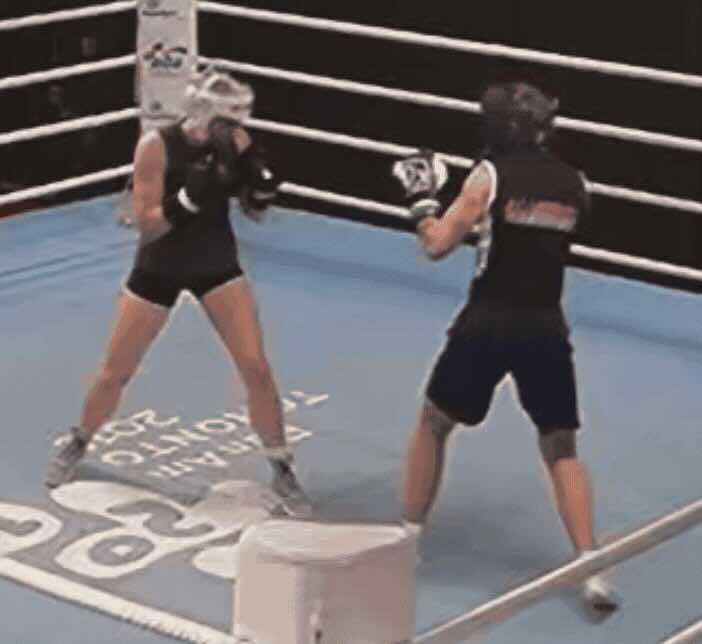
\includegraphics[height=5cm]{figures/p1.jpg}};
  \node[imagenode] (vdots) at (-4,-0.4)   {\vdots};
  \node[imagenode] (view2) at (-4,-1.4)  {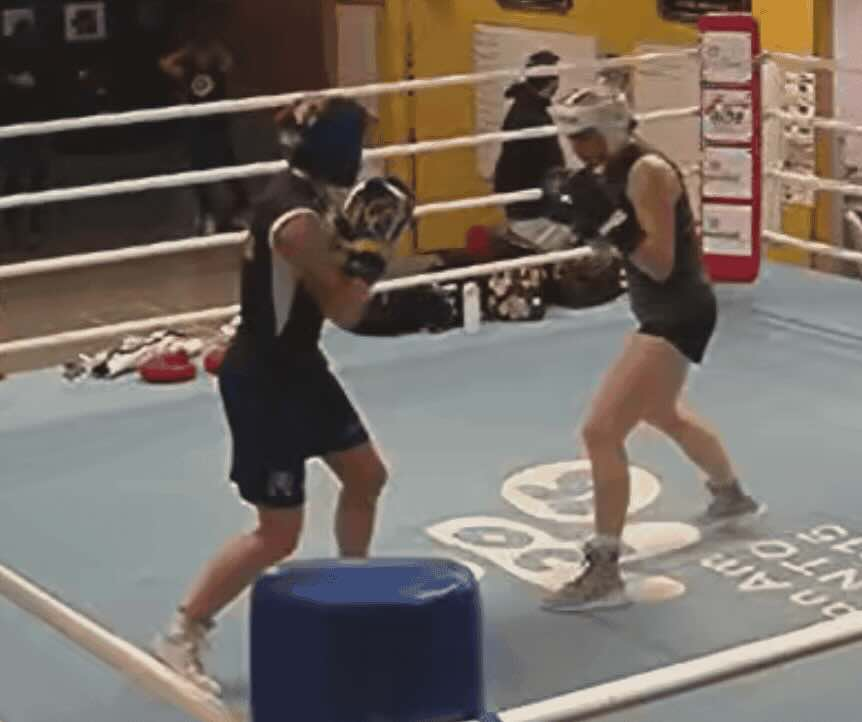
\includegraphics[height=5cm]{figures/p2.jpg}};

  % ─── pipeline stages on the same horizontal line ───────────────
  \node[process3] (yolo)    at (-2,-0.4) {Yolov8};
  \node[process3] (xmem)    at ( -1,-0.4) {XMem};
  \node[process3] (epi)    at ( 0,-0.4) {Epipolar Constraints};
  \node[process3] (vitpose) at ( 1,-0.4) {ViTPose};
  \node[imagenode] (tri)    at ( 4,-0.4) {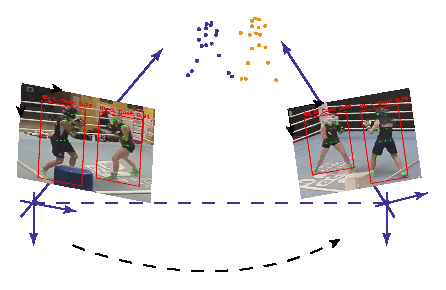
\includegraphics[height=9cm]{figures/triangulation}};
  \node[process]  (kin)     at ( 8.5,-0.4) {Kinematics\\Optimization};

  % ─── arrows between those five stages ────────────────────────────
  \draw[vecArrow] (vdots)   tonode[anchor=west, rotate=-90] {} (yolo);
  \draw[vecArrow] (yolo)    tonode[anchor=west, rotate=-90] {$\mathbf{bboxes}$} (xmem);
  \draw[vecArrow] (xmem)    tonode[anchor=west, rotate=-90] {$\mathbf{ids}$\cite{cheng2022xmem}} (epi);
  \draw[vecArrow] (epi)    tonode[anchor=west, rotate=-90] {sorted $\mathbf{ids}$\cite{wohler20093d}} (vitpose);
  \draw[vecArrow] (vitpose) tonode[anchor=west, rotate=-90] {$\mathbf{J}_{2D}$\cite{xu2022vitpose}} (tri);
  \draw[vecArrow] (tri)     -- (kin);

  % ─── auxiliary blocks above/below kinematics ────────────────────
  \node[process2] (prior) at ( 8.5, 0.8)  {GMM Prior, Vposer};
  \node[process2] (loss)  at ( 8.5,-1.8)  {$L_{2D},L_{3D},L_{\rm reg},L_{\rm smooth}$};
  \draw[vecArrow] (prior) -> (kin);
  \draw[vecArrow] (loss)  -> (kin);

  % ─── SMPL & downstream pipeline ────────────────────────────────
  \node[imagenode] (smpl2)   at (12,-0.4) {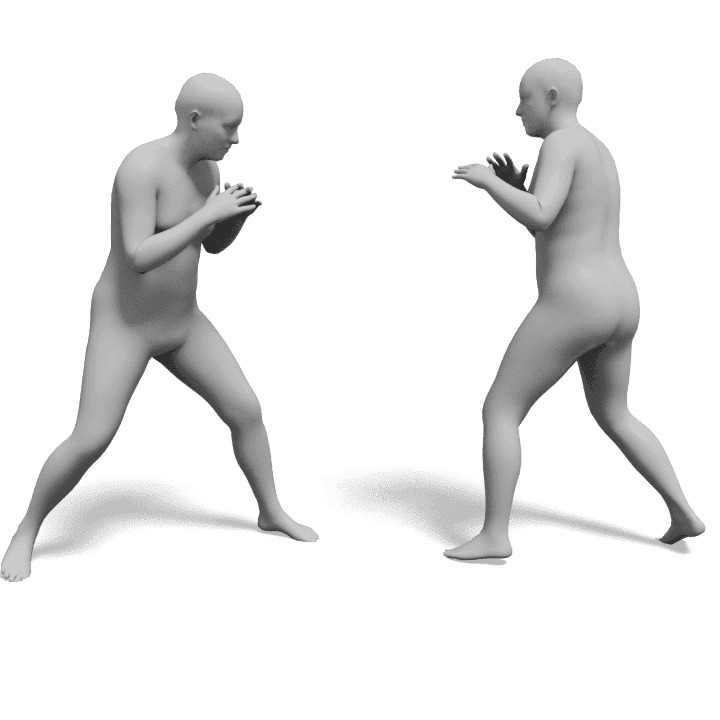
\includegraphics[height=7cm]{figures/smpl2.jpg}};
  \draw[vecArrow] (kin)   -- (smpl2);

  \node[imagenode] (smpl)   at (-4,-4)   {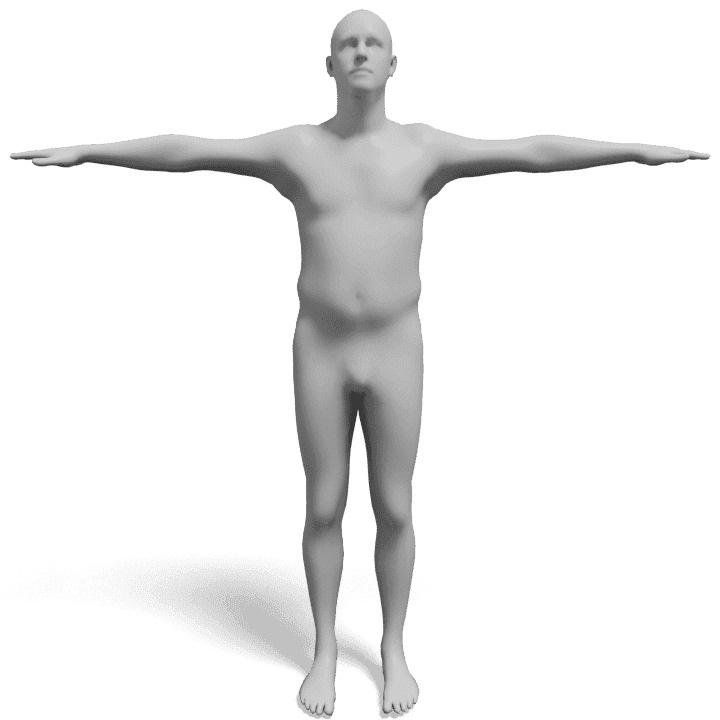
\includegraphics[height=7cm]{figures/smpl-tall.jpg}};
  \node[decision] (retarget) at (0.0,-4.0) {Physics Body Model Generator};
  \draw[vecArrow] (smpl)      -- (retarget);

  \node[imagenode] (hum)    at (3.5,-4.0) {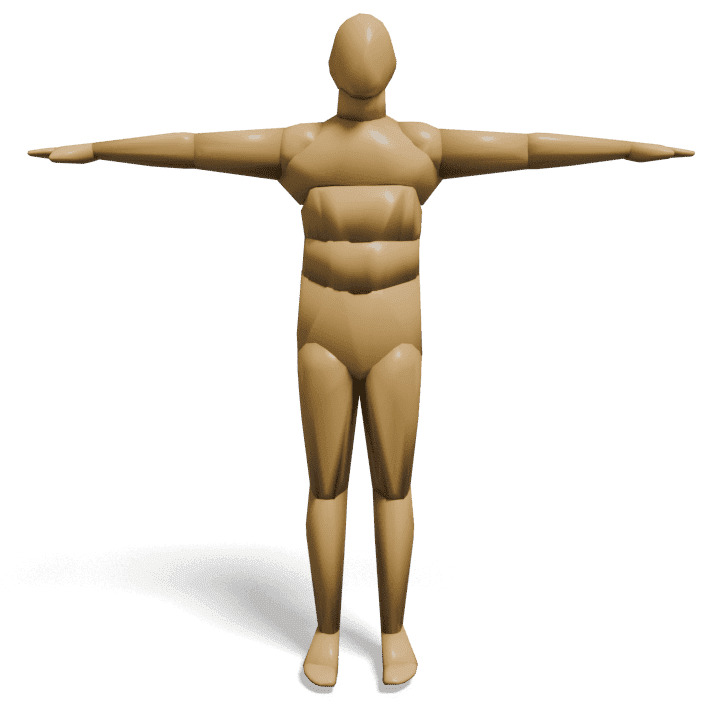
\includegraphics[height=7cm]{figures/humanoid-tall.jpg}};
  \draw[vecArrow] (retarget) -- (hum);

  \node[process] (lqr)      at (7.5,-4.0)  {Multi-Person iLQR Optimization};
  \draw[vecArrow] (hum)     -- (lqr);

  \draw[vecArrow]
     (smpl2.south)
       -- ++(0,-5cm)
       -- ++(-15.5cm,0)
       -- ++(0,-2.5cm)
       -- (lqr.north);

  \node[imagenode] (final) at (12,-4)   {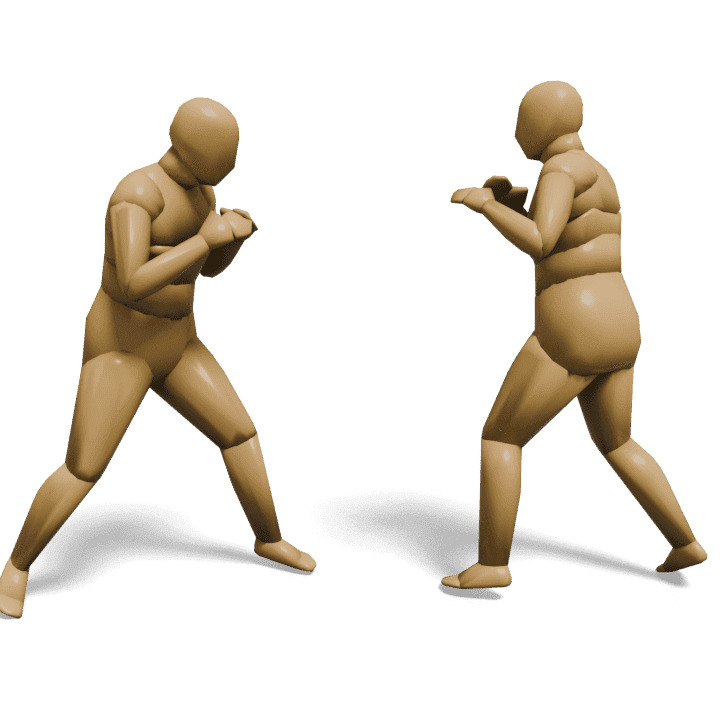
\includegraphics[height=7cm]{figures/final.jpg}};
  \draw[vecArrow] (lqr) -- (final);

\end{tikzpicture}
